\documentclass{wissdoc}
%\documentclass[oneside]{wissdoc}
% ----------------------------------------------------------------
% Diplomarbeit - Hauptdokument
% ----------------------------------------------------------------
% wissdoc Optionen: draft, relaxed, pdf, oneside --> siehe wissdoc.cls
% ------------------------------------------------------------------
% Packages für Deckblatt
\usepackage[absolute]{textpos} 	%Textboxen an absolute Position setzen
\usepackage{setspace}						%Zeilenabstand anpassen
\usepackage{color}							%Farbige Schrift
\usepackage{graphicx}						%Einbinden von Grafiken

% Weitere packages: (Dokumentation dazu durch "latex <package>.dtx")
% \usepackage{varioref}
% \usepackage{verbatim}
% \usepackage{float}    %z.B. \floatstyle{ruled}\restylefloat{figure}
\usepackage{subfigure}
\usepackage[ngerman]{babel}
\usepackage[T1]{fontenc}
\usepackage[ansinew]{inputenc}
\usepackage{tabularx}

\usepackage{float}

% ----------------------------------------------------------------------
% used for code examples
\usepackage{listings}

\definecolor{lightgray}{rgb}{.9,.9,.9}
\definecolor{darkgray}{rgb}{.4,.4,.4}
\definecolor{purple}{rgb}{0.65, 0.12, 0.82}


\renewcommand\lstlistingname{Quelltext} % Change language of section name
\usepackage{xcolor}
\lstset{ % General setup for the package
	language=bash,
	basicstyle=\small\sffamily,
	backgroundcolor=\color{lightgray},
	numbers=left,
	numberstyle=\tiny,
	frame=tb,
	tabsize=4,
	columns=fixed,
	showstringspaces=false,
	showtabs=false,
	keepspaces,
	commentstyle=\color{red},
	keywordstyle=\color{blue}
}


\lstdefinelanguage{JavaScript}{
	keywords={typeof, new, true, false, catch, function, return, null, catch, switch, var, if, in, while, do, else, case, break},
	keywordstyle=\color{blue}\bfseries,
	ndkeywords={class, export, boolean, throw, implements, import, this},
	ndkeywordstyle=\color{darkgray}\bfseries,
	identifierstyle=\color{black},
	sensitive=false,
	comment=[l]{//},
	morecomment=[s]{/*}{*/},
	commentstyle=\color{purple}\ttfamily,
	stringstyle=\color{red}\ttfamily,
	morestring=[b]',
	morestring=[b]"
}

\lstset{
	language=JavaScript,
	backgroundcolor=\color{lightgray},
	extendedchars=true,
	basicstyle=\footnotesize\ttfamily,
	showstringspaces=false,
	showspaces=false,
	numbers=left,
	numberstyle=\footnotesize,
	numbersep=9pt,
	tabsize=2,
	breaklines=true,
	showtabs=false,
	captionpos=b
}
% ----------------------------------------------------------------------

% Zeilenabstand nach Vorgabe - Falls gefordert
%\setstretch{1,3} 

% Inhaltsangabe auf Unterabschnitte(2 Ebenen) begrenzen
\setcounter{tocdepth}{2}


% \usepackage{color}    % Farbiger/grauer Text
% \usepackage{colortbl}   % Farbige/graue Tabellenzeilen und -spalten!! <--
% \usepackage{fancybox} % für schattierte,ovale Boxen etc.
% \usepackage{tabularx} % automatische Spaltenbreite
% \usepackage{supertab} % mehrseitige Tabellen
%% ---------------- end of usepackages -------------

%% Informationen für die PDF-Datei
\hypersetup{pdfauthor={Max Mustermann},%
            pdftitle={Bachelorarbeit},%
            pdfsubject={Titel der Arbeit},%
            pdfkeywords={Forschung, Entwicklung, Funktechnik},%
            pdfproducer={LaTeX},%
            pdfcreator={pdfLaTeX}
}

% Macros, nicht unbedingt notwendig
%%%%%%%%%%%%%%%%%%%%%%%%%%%%%%%%%%%%%%%%%%%%%%%%%%%%%%%%%%
% macros.tex -- einige mehr oder weniger nuetzliche Makros
%%%%%%%%%%%%%%%%%%%%%%%%%%%%%%%%%%%%%%%%%%%%%%%%%%%%%%%%%%


%%%%%%%%%%%%%%%%%%%%%%%
% Kommentare 
%%%%%%%%%%%%%%%%%%%%%%%
\ifnotdraftelse{
\newcommand{\Kommentar}[1]{}
}{\newcommand{\Kommentar}[1]{{\em #1}}}
% Alles innerhalb von \Hide{} oder \ignore{} 
% wird von LaTeX komplett ignoriert (wie ein Kommentar)
\newcommand{\Hide}[1]{}
\let\ignore\Hide

%%%%%%%%%%%%%%%%%%%%%%%%%
% Leere Seite ohne Seitennummer, wird aber gezaehlt
%%%%%%%%%%%%%%%%%%%%%%%%%

\newcommand{\leereseite}{% Leerseite ohne Seitennummer, n�chste Seite rechts (wenn 2-seitig)
 \clearpage{\pagestyle{empty}\cleardoublepage}
}

%%%%%%%%%%%%%%%%%%%%%%%%%%
% Neue Seite rechts, leere linke Seite ohne Headings
%%%%%%%%%%%%%%%%%%%%%%%%%%
\newcommand{\xcleardoublepage}
{{\pagestyle{empty}\cleardoublepage}}

%%%%%%%%%%%%%%%%%%%%%%%%%%
% Tabellenspaltentypen (benoetigt colortbl)
%%%%%%%%%%%%%%%%%%%%%%%%%%
\newcommand{\PBS}[1]{\let\temp=\\#1\let\\=\temp}
\newcolumntype{y}{>{\PBS{\raggedright\hspace{0pt}}}p{1.35cm}}
\newcolumntype{z}{>{\PBS{\raggedright\hspace{0pt}}}p{2.5cm}}
\newcolumntype{q}{>{\PBS{\raggedright\hspace{0pt}}}p{6.5cm}}
\newcolumntype{g}{>{\columncolor[gray]{0.8}}c} % Grau
\newcolumntype{G}{>{\columncolor[gray]{0.9}}c} % helleres Grau

%%%%%%%%%%%%%%%%%%%%%%%%%%
% Anf�hrungszeichen oben und unten
%%%%%%%%%%%%%%%%%%%%%%%%%%
\newcommand{\anf}[1]{"`{#1}"'}

%%%%%%%%%%%%%%%%%%%%%%%%%%
% Tiefstellen von Text
%%%%%%%%%%%%%%%%%%%%%%%%%%
% S\tl{0} setzt die 0 unter das S (ohne Mathemodus!)
% zum Hochstellen gibt es uebrigens \textsuperscript
\makeatletter
\DeclareRobustCommand*\textlowerscript[1]{%
  \@textlowerscript{\selectfont#1}}
\def\@textlowerscript#1{%
  {\m@th\ensuremath{_{\mbox{\fontsize\sf@size\z@#1}}}}}
\let\tl\textlowerscript
\let\ts\textsuperscript
\makeatother

%%%%%%%%%%%%%%%%%%%%%%%%%%
% Gau�-Klammern
%%%%%%%%%%%%%%%%%%%%%%%%%%
\newcommand{\ceil}[1]{\lceil{#1}\rceil}
\newcommand{\floor}[1]{\lfloor{#1}\rfloor}

%%%%%%%%%%%%%%%%%%%%%%%%%%
% Average Operator (analog zu min, max)
%%%%%%%%%%%%%%%%%%%%%%%%%%
\def\avg{\mathop{\mathgroup\symoperators avg}}

%%%%%%%%%%%%%%%%%%%%%%%%%%
% Wortabk�rzungen
%%%%%%%%%%%%%%%%%%%%%%%%%%
\def\zB{z.\,B.\ }
\def\dh{d.\,h.\ }
\def\ua{u.\,a.\ }
\def\su{s.\,u.\ }
\newcommand{\bzw}{bzw.\ }

%%%%%%%%%%%%%%%%%%%%%%%%%%%%%%%%%%%
% Einbinden von Graphiken
%%%%%%%%%%%%%%%%%%%%%%%%%%%%%%%%%%%
% global scaling factor
\def\gsf{0.9}
%% Graphik, 
%% 3 Argumente: Datei, Label, Unterschrift
\newcommand{\Abbildung}[3]{%
\begin{figure}[tbh] %
\centerline{\scalebox{\gsf}{\includegraphics*{#1}}} %
\caption{#3} %
\label{#2} %
\end{figure} %
}
\let\Abb\Abbildung
%% Abbps
%% Graphik, skaliert, Angabe der Position
%% 5 Argumente: Position, Breite (0 bis 1.0), Datei, Label, Unterschrift
\newcommand{\Abbildungps}[5]{%
\begin{figure}[#1]%
\begin{center}
\scalebox{\gsf}{\includegraphics*[width=#2\textwidth]{#3}}%
\caption{#5}%
\label{#4}%
\end{center}
\end{figure}%
}
\let\Abbps\Abbildungps
%% Graphik, Angabe der Position, frei w�hlbares Argument f�r includegraphics
%% 5 Argumente: Position, Optionen, Datei, Label, Unterschrift
\newcommand{\Abbildungpf}[5]{%
\begin{figure}[#1]%
\begin{center}
\scalebox{\gsf}{\includegraphics*[#2]{#3}}%
\caption{#5}%
\label{#4}%
\end{center}
\end{figure}%
}
\let\Abbpf\Abbildungpf

%%
% Anmerkung: \resizebox{x}{y}{box} skaliert die box auf Breite x und H�he y,
%            ist x oder y ein !, dann wird das uspr�ngliche 
%            Seitenverh�ltnis beibehalten.
%            \rescalebox funktioniert �hnlich, nur das dort ein Faktor
%            statt einer Dimension angegeben wird.
%%
% \Abbps{Position}{Breite in Bruchteilen der Textbreite}{Dateiname}{Label}{Bildunterschrift}
%

\newcommand{\refAbb}[1]{%
s.~Abbildung \ref{#1}}

%%%%%%%%%%%%%%%%%%%%
%% end of macros.tex
%%%%%%%%%%%%%%%%%%%%

% Print URLs not in Typewriter Font
\def\UrlFont{\rm}

\newcommand{\blankpage}{% Leerseite ohne Seitennummer, nächste Seite rechts
 \clearpage{\pagestyle{empty}\cleardoublepage}
}

%% Einstellungen für das gesamte Dokument

% Trennhilfen
% Wichtig!
% Im german-paket sind zusätzlich folgende Trennhinweise enthalten:
% "- = zusätzliche Trennstelle
% "| = Vermeidung von Ligaturen und mögliche Trennung (bsp: Schaf"|fell)
% "~ = Bindestrich an dem keine Trennung erlaubt ist (bsp: bergauf und "~ab)
% "= = Bindestrich bei dem Worte vor und dahinter getrennt werden dürfen
% "" = Trennstelle ohne Erzeugung eines Trennstrichs (bsp: und/""oder)

% Trennhinweise fuer Woerter hier beschreiben
\hyphenation{
% Pro-to-koll-in-stan-zen
% Ma-na-ge-ment  Netz-werk-ele-men-ten
% Netz-werk Netz-werk-re-ser-vie-rung
% Netz-werk-adap-ter Fein-ju-stier-ung
% Da-ten-strom-spe-zi-fi-ka-tion Pa-ket-rumpf
% Kon-troll-in-stanz
}

%Tabellen Kommandos
\newcolumntype{L}[1]{>{\raggedright\arraybackslash}p{#1}}
\newcolumntype{C}[1]{>{\centering\arraybackslash}p{#1}}
\newcolumntype{R}[1]{>{\raggedleft\arraybackslash}p{#1}}

% Index-Datei öffnen
\ifnotdraft{\makeindex}
%%%%%%%%%%%%%% includeonly %%%%%%%%%%%%%%%%%%%
% Es werden nur die Teile eingebunden, die hier aufgefuehrt sind!
%\includeonly{%
%titelseite,%
%erklaerung,%
%kurzfassung,%
%einleitung,%
%analyse,%
%entwurf,%
%implemen,%
%zusammenf%
%}
%%%%%%%%%%%%%%%%%%%%%%%%%%%%%%%%%%%%%%%%%%%%%%
\begin{document}
%Auskommentiert, da nicht notwendig für das Praktikum
%\ifnotdraft{
	%%%%Vorlage
	% 
\thispagestyle{empty}
\begin{figure}[t]
		\hspace{-2.2cm}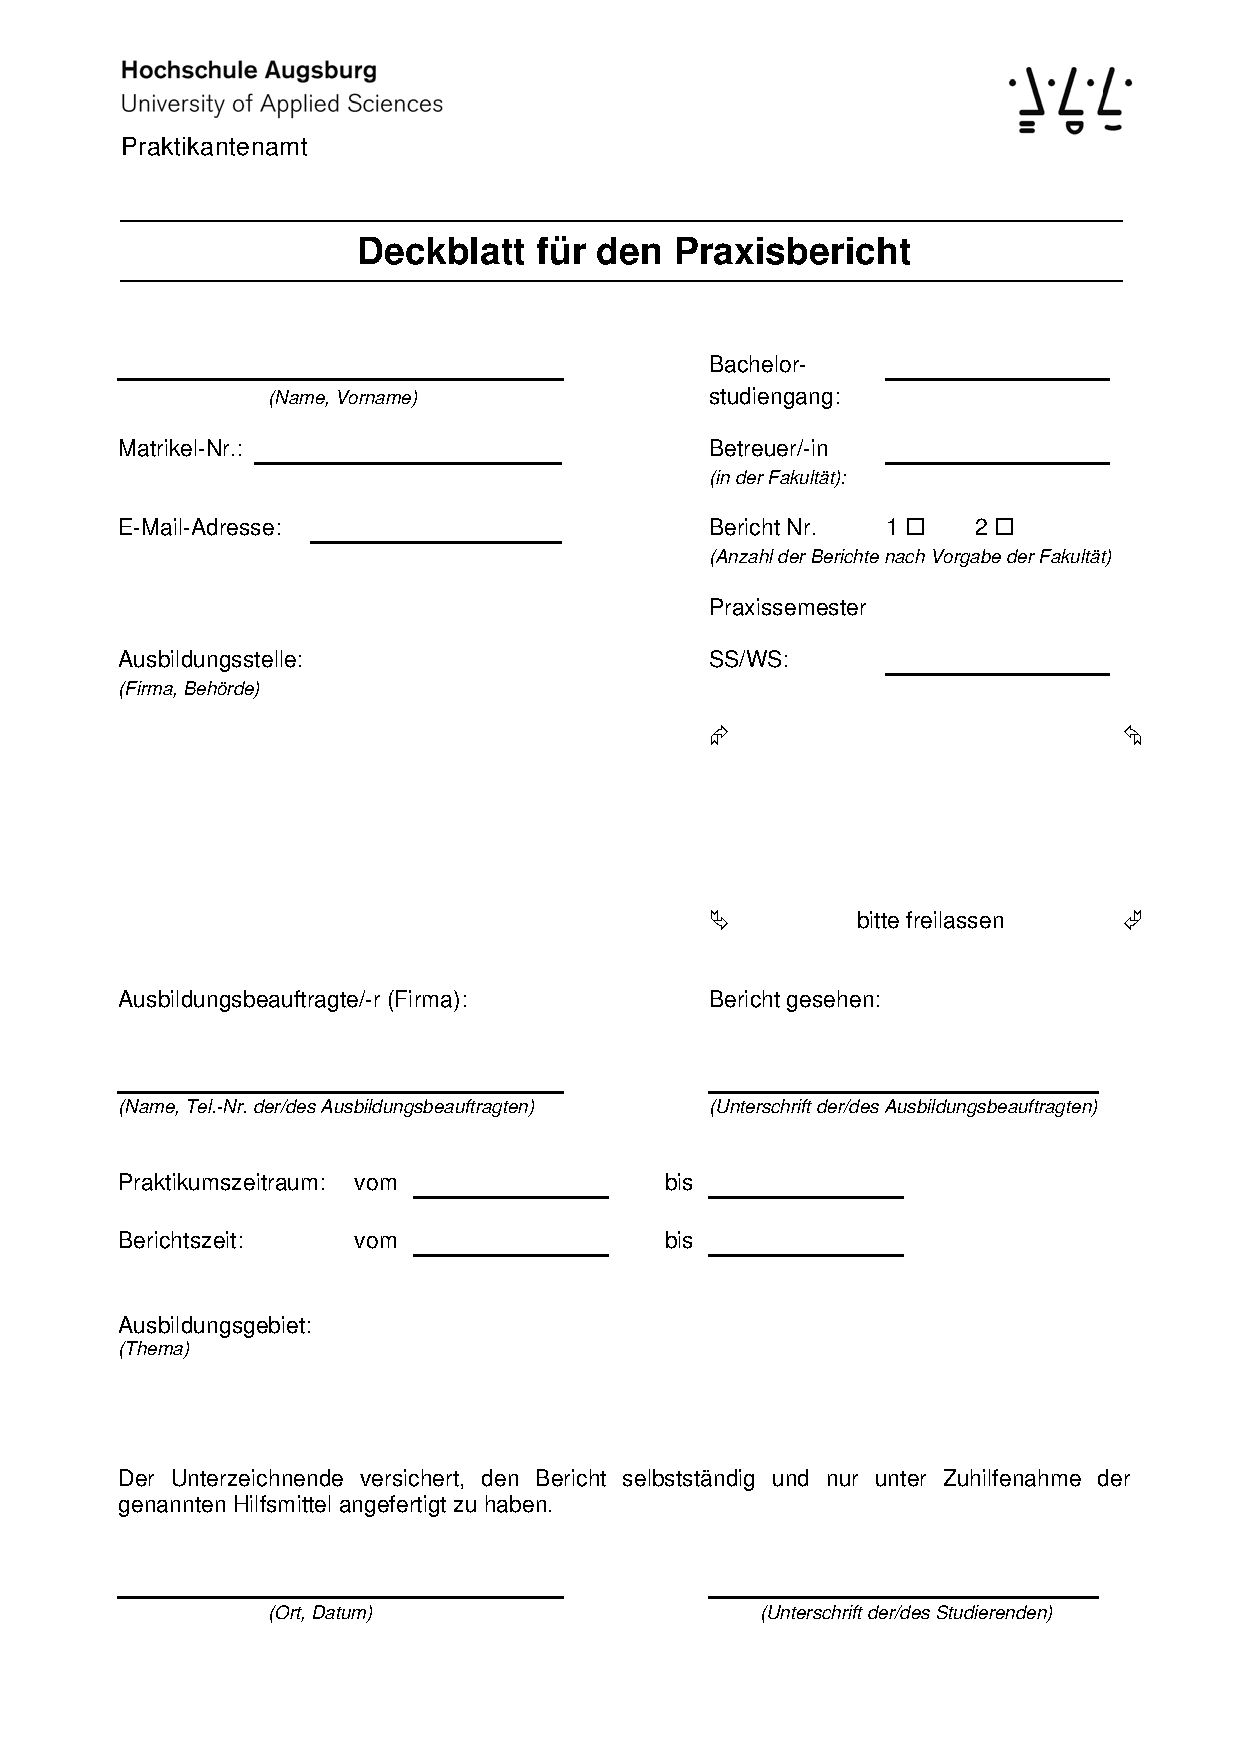
\includegraphics[width=0.93\paperwidth]{figures/deckblatt_prax_bac}
	\label{fig:deckblatt_prax_bac}
\end{figure}
  %<-- Nach Vorgabe der HS Augsburg

	%%% Deckblatt - Hochschule Augsburg
%%%Deckblatt

\textblockorigin{20mm}{30mm}

\thispagestyle{empty}\null
%%%%Logo - Hochschule Augsburg - Informatik
\begin{textblock}{10}(8.0,1.1)
\begin{figure}[h]
	\centering
		
\includegraphics[width=0.45\textwidth]{logos/hsa_informatik_logo_lq.pdf}
\end{figure}

\end{textblock}

%%% Text unter Logo
\begin{textblock}{15}(12.43,2.1)
	\LARGE
	\textsf{
		\textbf{\textcolor[rgb]{1,0.41,0.13}{\\
			\begin{flushleft}
				Fakult�t f�r\\
				Informatik\\
			\end{flushleft}
			}
		}
	}
\end{textblock}

%%%%Textbox links - Informationen
\begin{textblock}{15}(2,1.4)
	%\LARGE
	\begin{flushleft}
		\begin{spacing} {1.2}
			\huge	
				\textbf{Methoden der KI\\}
				\vspace{30pt}
				\textcolor[rgb]{1,0.41,0.13}{\\
				\textbf{Portfoliopr�fung}}\\
				\vspace{60pt}
			\LARGE
				Studienrichtung\\
				Technische Informatik\\
				\vspace{40pt}
				
				Muhammad Aman Bin Ahmad Tifli\\
				\vspace{30pt}		
				Matrikelnummer: 2042550\\
				% \vspace{30pt}		
				% Ausbildungsstelle: KUKA Deutschland AG\\
				\vspace{60pt}		
			\LARGE
				Pr\"ufer: Prof. Dr. Thomas Rist\\
				\vspace{10pt}		
				Abgabedatum: xx.xx.2021\\
			\end{spacing}
		\end{flushleft}
		
\end{textblock}



%%%%Textbox rechts - Hochschule
\begin{textblock}{5}(12.45,9.0)
	\scriptsize
	\textcolor[rgb]{1,0,0}{\\
		\begin{flushleft}
			\begin{spacing} {1.3}
				Hochschule f\"ur angewandte\\
				Wissenschaften Augsburg\\
				\vspace{4pt}
				An der Hochschule 1\\
				D-86161 Augsburg\\
				\vspace{4pt}
				Telefon +49 821 55 86-0\\
				Fax +49 821 55 86-3222\\
				www.hs-augsburg.de\\
				info(at)hs-augsburg-de
			\end{spacing}
		\end{flushleft}
		}
\end{textblock}


%%%%Textbox rechts unten - Fakult?t und Autor
\begin{textblock}{5}(12.45,11.5)
	\scriptsize
		\begin{flushleft}
			\begin{spacing} {1.3}
				Fakult\"at f\"ur Informatik\\
				Telefon +49 821 55 86-3450\\
				Fax \hspace{10pt} +49 821 55 86-3499\\
				\vspace{6pt}
				Verfasser der Diplomarbeit\\
				Max Mustermann\\
				Beispielstra?e 31\\
				86150 Augsburg\\
				Telefon +49 821 55 86-3450\\
				max@hs-augsburg.de\\
			\end{spacing}
		\end{flushleft}
	\end{textblock}
\pagebreak  %<-- Nach Vorgabe der HS Augsburg
	%
	%%%% Innere Titelseite 
 	%\include{titelseite} %<-- Vorgabe Prüfer oder frei wählbar
	%
	%%%%Optional - Falls von der Firma gefordert
	%\include{sperrvermerk}
	%
	%%%%Pflicht
 	%\include{erklaerung}
	%
	%%% Leere Seite bei zweiseitigem Druck
	%\ifnotonesideelse{\blankpage}{}
	%\include{kurzfassung}
	%%% Leere Seite bei zweiseitigem Druck
	%\ifnotonesideelse{\blankpage}{}
%}



%
%% ++++++++++++++++++++++++++++++++++++++++++
%% Verzeichnisse
%% ++++++++++++++++++++++++++++++++++++++++++
\pagenumbering{roman}
\ifnotdraft{
\tableofcontents
% Leere Seite bei zweiseitigem Druck
%\ifnotonesideelse{\blankpage}{}
%\listoffigures
%% Leere Seite bei zweiseitigem Druck
%\ifnotonesideelse{\blankpage}{}
%\listoftables
%% Leere Seite bei zweiseitigem Druck
%\ifnotonesideelse{\blankpage}{}
}
%% ++++++++++++++++++++++++++++++++++++++++++
%% Hauptteil
%% ++++++++++++++++++++++++++++++++++++++++++
\graphicspath{{figures/}}
\pagenumbering{arabic}

%%% Ab hier eigene Kapitel einfügen
%%% Kapitel sind analog zur Wordvorlage zu wählen

\chapter{Introduction}
\chapter{Formulierung von Problemen und Lösungen in der Symbolischen Informationsverarbeitung}
\chapter{Probleml�sung als Suchaufgabe}

\section{Wegsuche ohne Karte}

``Wegsuche ohne Karte'' bedeutet Wegfindung in einer unbekannten Umgebung ohne eine Karte, die den Agenten leitet.

Beispiel: \textbf{Roboter R} befindet sich in einem unbekannten Gebiet und muss sich zu einem Zielobjekt bewegen. Dies kann durch Anwendung eines \textbf{Bug-Algorithmus} gel�st werden, der voraussetzt, dass der Roboter mit Sensoren ausgestattet ist, um Hindernisse und das \textbf{Zielobjekt S} zu erkennen.

\subsection{Bug Algorithmen Beispiel}
\label{bug-algo-1}
Ein Beispiel f�r einen Bug-Algorithmus ist wie folgt:
\begin{enumerate}
    \item Wenn das \textbf{Zielobjekt S} in Sichtweite ist, fahrt \textbf{Roboter R} direkt darauf zu
    \item Wenn \textbf{S} nicht in Sicht ist, aber stattdessen ein Hindernis vorhanden ist, bewegt sich \textbf{R} gem�� einer bestimmten Regel um das Hindernis herum (z. B. im Uhrzeigersinn).
    \item \textbf{R} scannt erneut nach dem Objekt \textbf{S} und wiederholt die Schritte 1 und 2, bis das Ziel erreicht ist.
\end{enumerate}

\begin{figure}[H]
    \centering
    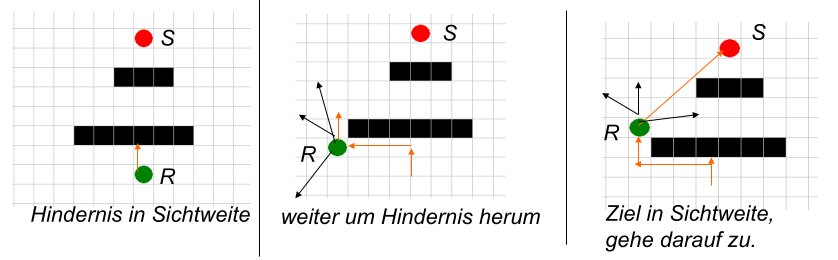
\includegraphics[width=\textwidth]{figures/kap3/bug-algo-1.png}
    \caption{Beispiel von Bug-Algorithmus Verfahren}
    \label{fig:bug-algo}
\end{figure}

\subsection{Problem mit dem Bug-Algorithmus}

In bestimmten Situationen (z.B siehe Abb. \ref{fig:bug-algo-prob}) ist der Roboter mit dem Ansatz in Abschnitt~\ref{bug-algo-1} nicht in der Lage, das Ziel zu finden.

\begin{figure}[H]
    \centering
    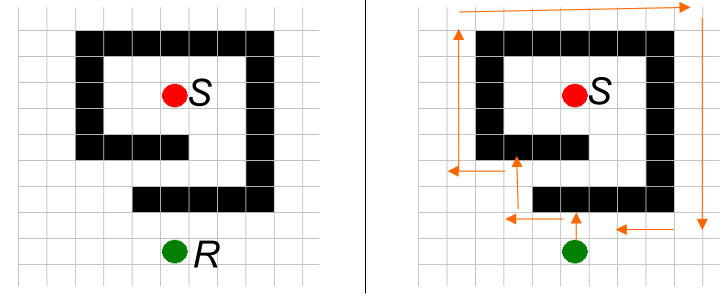
\includegraphics[width=0.8\textwidth]{figures/kap3/bug-algo-1-problem.png}
    \caption{Der Roboter kann das Ziel nicht sehen}
    \label{fig:bug-algo-prob}
\end{figure}

Der Algorithmus muss verbessert werden, z. B. durch Bewegen gegen den Uhrzeigersinn, um eine Bewegung in einem kontinuierlichen Kreis zu vermeiden.

\begin{figure}[H]
    \centering
    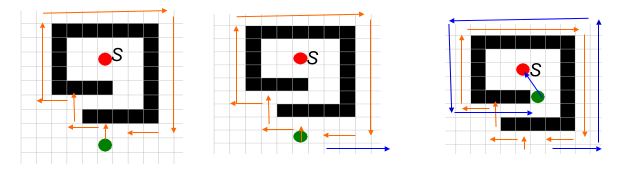
\includegraphics[width=\textwidth]{figures/kap3/bug-algo-1-fix.png}
    \caption{Gegen den Uhrzeigersinn bewegen, um das Ziel zu erreichen}
    \label{fig:bug-algo-fix}
\end{figure}

\section{Repr�sentation von Suchr�umen}

\subsection{Suchraum als Karte}

Ein Suchraum wird normalerweise als grafische Karte dargestellt. Diese Karten k�nnen als Wegenetz oder als Gitter mit benachbarten Zellen dargestellt werden, wie in Abbildung \ref{fig:graph-examples} gezeigt.

\begin{figure}[H]
    \centering
    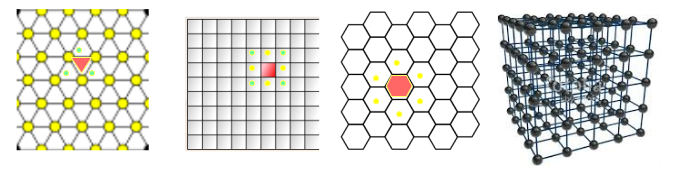
\includegraphics[width=\textwidth]{figures/kap3/graph-examples.png}
    \caption{Beispiele von Gittermustern}
    \label{fig:graph-examples}
\end{figure}

Je nach verwendetem Gittermuster werden unterschiedliche Suchgraphen basierend auf der Anzahl der Nachbarn jeder Zelle im Gitter gebildet. Zum Beispiel: Eine dreieckige Zelle hat sechs Nachbarn, eine quadratische Zelle hat 4 (oder 8, wenn Diagonalen erlaubt sind) und eine sechseckige Zelle hat 6.

\section{Wegsuche als systemstisches Ablaufen von Graphen}

Bei der Wegfindung mit Hilfe eines Graphen m�ssen ein \textbf{Startknoten} und eine \textbf{Funktion zum Testen}, ob der Zielknoten erreicht wurde, definiert werden. Mit Hilfe des Startknotens und dieser Funktion kann eine Folge von Knoten gefunden werden, die die Testfunktion erf�llen k�nnen. Wichtig ist, dass die f�r die Sequenz ausgew�hlten Knoten \textbf{benachbarte Knoten sind, die durch Kanten verbunden} sind.

\subsection{Expliziter Graphen und sukzessive Expansion}

Es ist wichtig, zwischen einem expliziten Graphen und einem ``gedachten'' Graphen als Repr�sentation eines Suchraums f�r L�sungen zu unterscheiden.

\paragraph{Expliziter Graphen}

Eine explizite Darstellung der Knoten und Kanten ist verf�gbar (z.B Adjazentmatrix). Dies ist nur f�r kleinere Knotenmengen praktikabel und die meisten Probleme erfordern keine vollst�ndige Repr�sentation des Suchgraphen.

\paragraph{Sukzessive Expansion}

Diagramm ist verf�gbar, aber nicht vollst�ndig explizit. Der Suchprozess erfolgt durch Knotenerweiterung, indem Knoten f�r Knoten vorgegangen wird.

\subsection{Generelle Wegfindungsstrategie}

Zyklen und Mehrfachbesuche sind zu vermeiden, da sie den Suchbaum exponentiell wachsen lassen k�nnen. Generell sollte man keinen bereits benutzten Weg nochmal gehen, keine Wege mit Zyklen kreieren, einen bereits besuchten oder ausgebauten Zustand nicht nochmal besuchen oder erzeugen.

\subsection{Generelle Bewertung von S uchverfahren} 

Bewertungskriterien eines Pfadfindungsprozesses sind wie folgt:

\paragraph{Korrektheit}

Es ist wichtig, dass die Wegfindungsl�sung tats�chlich eine L�sung des Problems ist.

\paragraph{Vollst�ndigkeit}

Existiert eine L�sung, terminiert der Algorithmus nach endlicher Zeit und generiert eine L�sung.

\paragraph{Optimalit�t}

Die optimalste L�sung wird gefunden, wenn mehrere m�glich sind.

\paragraph{Zeitkomplexit�t}

Die Zeit, die im worst-case/average-case ben�tigt wird, um eine optimale L�sung zu finden.

\paragraph{Speicherkomplexit�t}

Wie viel Speicher, die im worst-case/average-case ben�tigt wird.



\section{Arten von Suchverfahren}

Es gibt viele M�glichkeiten, eine Wegfindungssuche durchzuf�hren. Diese n�chsten Abschnitte werden darauf eingehen.

\subsection{Breitensuche in expliziten Graphen}
\label{section:breitensuche}
Breitensuche ist auf Englisch ``breadth first search''. F�r diesen Algorithmus werden f�r jeden Knoten zus�tzliche Daten ben�tigt: \textbf{noch nicht gesucht} (wei� dargestellt), \textbf{entdeckt, aber noch nicht verarbeitet } (grau dargestellt), \textbf{verarbeitet} (schwarz dargestellt). 

\paragraph{�berblick �ber den Ablauf:}

\begin{enumerate}
    \item W�hle einen Startknoten aus dem Graphen und legen Sie diesen in die Warteschlange, Q. Alle Knoten in Q sind grau markiert.
    \item Solange es Elemente in Q gibt, markiere alle Nachbarn der Elemente grau und f�ge diese der Warteschlange Q hinzu. 
    \item Nachdem alle Nachfolger eines Knotens grau markiert wurden, markiere den Knoten schwarz und entferne ihn aus der Warteschlange. Pr�fen Sie, w�hrend Sie die Nachfolgerknoten grau markieren, ob der zu markierende Knoten der Zielknoten ist.s
    \item Wiederhole Schritt 2 und Schritt 3, bis die Warteschlange Q leer ist.
\end{enumerate}

\paragraph{Komplexit�tsbetrachtung}

Speicherbedarf und Zeitbedarf sind exponentiell. Dies f�hrt dazu, dass gro�e Graphen unl�sbar sind und sogar relativ kleine Graphen zu lange brauchen, um praktikabel zu sein (z.B Graphen Tiefe 12 brauch 35 Jahre Rechenzeit).

\subsection{Uniforme Kostensuche}

Bei diesem Suchalgorithmus wird die Breitensuche so ver�ndert, dass auch die \textbf{Kosten der Nachbarknoten} ber�cksichtigt werden. Da die Kosten zweier benachbarter Knoten normalerweise bereits bekannt sind, kann \textbf{die Warteschlange in einen Heap umstrukturiert werden}, der in \textbf{aufsteigender Reihenfolge der Pfadkosten} sortiert ist. Auf diese Weise wird gehofft, dass der k�rzeste Weg vom Startknoten zum Zielknoten gefunden wird.

\subsection{Modifizierte Uniforme Kostensuche / Dijkstra}

Um eine optimale L�sung f�r ein Wegsucheproblem zu finden, ist es notwendig, alternative Pfade parallel zu konstruieren. Wenn sich diese Pfade am selben Punkt treffen, kann der \textbf{k�rzeste Pfad beibehalten werden}, w�hrend der Rest aus dem Suchbaum entfernt wird, um die k�rzeste Gesamtroute zu finden.

Wenn ein Pfad zum Zielknoten gefunden wird, werden alle \textbf{anderen parallelen Pfade fortgesetzt}, es sei denn, ihre Kosten �bersteigen den bereits gefundenen Pfad. Dies f�hrt zu einer besseren Effizienz bei der Suche nach dem k�rzesten Weg. 

\begin{figure}[H]
    \centering
    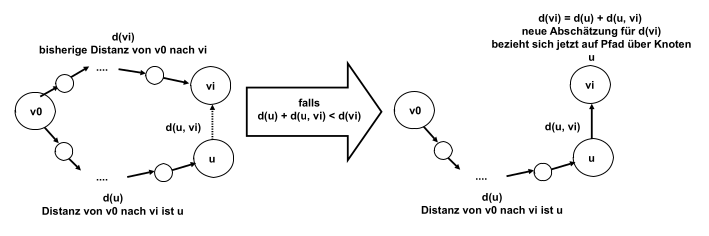
\includegraphics[width=\textwidth]{figures/kap3/dijkstra.png}
    \caption{Dijkstra-Algorithmus Pfadsuche}
    \label{fig:graph-dijkstra}
\end{figure}

Dieser Algorithmus ist in Abbildung \ref{fig:graph-dijkstra} demonstriert. Anhand der Abbildung kann man sehen, wie die beiden Routen von v0 nach vi verglichen werden und die Kosten verglichen werden, um nur die k�rzere Route beizubehalten.

\subsection{Ablauf eines Graphen mit Tiefensuche}

Im Gegensatz zur Traversierung mit Breitensuche verl�uft die Traversierung mit Tiefensuche auf m�glichst langen Wegen und f�hrt die Wei�-Grau-Schwarz-Markierung (siehe Abschnitt \ref{section:breitensuche}) durch. Dieser Algorithmus wird normalerweise rekursiv implementiert.

\paragraph{Ablauf von Tiefensuche}

\begin{enumerate}
    \item W�hle einen Startknoten \( v_s \). Markiere den Knoten als grau ein.
    \item F�r jeden Nachbarknoten \( v_k \) von \( v_s \), der wei� markiert ist, f�hre folgendes durch:
    \begin{enumerate}
        \item F�ge \( v_k \) zum Stack hinzu
        \item Markiere \( v_k \) als grau
        \item Falls \( v_k \) Nachbarn hat, f�hre Schritt (2) rekursiv aus
        \item Wenn \( v_k \) keine Nachbarn hat oder seine Nachbarn schwarz markiert sind, markiere \( v_k \) schwarz und entferne \( v_k \) vom Stack
    \end{enumerate}
    \item Der Algorithmus endet, sobald der Stack leer ist.
\end{enumerate}

\paragraph{Komplexit�tsbetrachtung}

Nur benachbarte Knoten des aktuellen Suchpfads werden auf dem Stack gespeichert. Dies bedeutet viel weniger Knotenerweiterungen im Vergleich zur Breitensuche, was zu weniger Speicherverbrauch f�hrt. Die Zeitkomplexit�t ist jedoch ebenso wie die Brreitensuche exponentiell.

\subsection{Tiefensuche und Backtracking-Algorithmen}

In realen Anwendungen beinhaltet eine L�sung die Verwendung vieler verschiedener Komponenten. Die endg�ltige L�sung verwendet daher normalerweise viele Teill�sungen, die m�glicherweise nicht richtig erweitert werden k�nnen (z.B: erreicht die Teill�sung eine Sackgasse). In diesen F�llen muss die Teill�sung durch eine weniger komplexe L�sung ersetzt werden.

\paragraph{Genereller Ablauf von einem Backtracking-Algorithmus}

Gegeben sind ein Array ``SolutionComponents'', das alle Werte der endg�ltigen L�sung enth�lt, und die Funktionen ``FirstTrialValue()'', ``NextTrialValue()'' und ``CheckValid()''.

\begin{enumerate}
    \item Der ersten Komponente wird der erste Versuchswert gegeben:\\~\\
    \lstinline{SolutionComponents[0] = FirstTrialValue(0)}~\\
    \item Die G�ltigkeit der L�sung wird �berpr�ft:\\~\\
    \lstinline{CheckValid(SolutionComponents)}~\\
    \item Wenn die bisherige L�sung g�ltig ist, fahren Sie mit dem n�chsten Wert fort (i = 1, 2, 3...) und �berpr�fe den Wert erneut\\~\\
    \lstinline{SolutionComponents[i] = FirstTrialValue(i)}~\\
    \lstinline{CheckValid(SolutionComponents)}~\\
    \item Wenn der CheckValid-Funktion an einem bestimmten Punkt false zur�ckgibt, versuche es mit den n�chsten Werten. Wenn alle Werte ebenfalls falsch zur�ckgeben, f�hre ein Backtracking durch, indem Sie i um i reduzieren und den n�chsten Wert f�r dieses i versuchen.Erh�hen Sie dann i wieder um 1 und probieren Sie alle Werte aus.
    \item Schritt 4 wird so oft wie n�tig wiederholt. F�r den Fall, dass i null erreicht und es keine Versuchswerte mehr f�r i = 0 gibt, gibt es keine m�gliche L�sung.
\end{enumerate}

\subsection{Limitierte Tiefensuche}

Es ist m�glich, die Nachteile der Tiefensuche zu vermeiden, indem man eine maximale Tiefe des Pfades einstellt. Das macht die Suche vollst�dnig aber nicht immer optimal. Um diese Idee zu erweitern, kann eine iterative Tiefensuche versucht werden. 

\subsection{Iterative Tiefensuche}

Bei dieser Methode wird die Tiefe mit jeder Iteration erh�ht, um sicherzugehen, dass eine L�sung gefunden wird.

\subsection{Bidirektionale Suche}

Anstatt nur vom Startknoten aus zu beginnen, f�hren Sie eine Suche vom Start- und vom Zielknoten aus durch. Wenn sich die beiden Verfahren in der Mitte treffen, ist eine L�sung gefunden.

\section{KI-Suchverfahren}

Es gibt zwei Klassen von Suchverfahren: \textbf{blinde Suchverfahren} und \textbf{KI-Suchverfahren}. Blinde Suchverfahren sind auf einem bestimmten Schema basiert, das unabh�ngig von dem jeweiligen Problem ist. Einige Beispiele hierf�r sind die in den vorangegangenen Kapiteln behandelten Verfahren wie Breitensuche, Tiefensuche, Biridketionale Suche usw. 

KI-Suchverfahren hingegen nutzen problemspezifisches Vorwissen zur Eingrenzung des Suchraums. Es handelt sich um informierte heuristische Suchverfarhen.

\textbf{Blinde Suchverfahren} erfordern, dass eine L�sung durch systematische und ersch�pfende Suche in einem Suchgraphen gefunden wird, was ineffizient und kein problemspezifisches Wissen nutzt.

\textbf{Informierte Suchprozesse} hingegen nutzen problemspezifische Eigenschaften, um die Effizienz der Knotenexpansion zu verbessern.

\subsection{Greedy Search}
\label{section:greedy-search}
Die Greedy-Suche ist eine modifizierte Breitensuche (siehe Abschnitt \ref{section:breitensuche}), bei der nur die Knoten mit den geringsten Kosten in die Warteschlange aufgenommen werden. 

\paragraph{Ablauf von Greedy Search}

Wenn die Kosten des aktuellen Knotens zum Zielknoten unbekannt sind, \textbf{m�ssen diese Kosten gesch�tzt werden}, und dann wird der Nachbar mit den geringsten Kosten ausgew�hlt. Die Funktion, die diese Kosten sch�tzt, wird \textbf{heuristische Funktion} genannt.

Der Unterschied zwischen Greedy Search und Uniform Cost Search (siehe Abschnitt \ref{section:uniform-cost-search}) besteht darin, dass bei der Greedy Search \textbf{die Kosten von einem Knoten zum Zielknoten} berechnet werden und nicht von einem Knoten zum anderen.

\paragraph{Eigenschaften von Greedy Search}

Greedy Search bietet tendenziell schnelle L�sungen, die oft, aber nicht immer, der optimale Weg sind. 

Greedy Search ist �hnlich wie die Tiefensuche mit Backtracking, nicht vollst�ndig, und erfordert eine gute Heuristik f�r eine bessere G�te des Verfahrens.

\subsection{Der A* Algorithmus}

Der A*-Algorithmus ist ein neuer Ansatz, der auf Greedy Search (Abbschnitt~\ref{section:greedy-search}) und dem Dijkstra-Algorithmus~(Abbschnitt~\ref{section:dijkstra}) aufbaut. A* arbeitet basierend auf der Funktion:

\[f(n) = g(n) + h(n)\]

Wobie \(f(n)\) die gesch�tzten Kosten der billigsten L�sung ist, \(g(n)\) die Kosten f�r die Bewegung von der Ausgangszelle zur aktuellen Zelle, und \(h(n)\) die gesch�tzten Kosten f�r die Bewegung von der aktuellen Zelle zur Zielzelle. Mit der Funktion \(f(n)\) werden die Kosten berechnet, und der Rest des Algorithmus l�uft wie bei Greedy Serach ab.

\subsection{Pfadplannung mit A*}

\subsection{Pfadplannung in Computerspielen}



\section{Vertiefungsprojekt: A*-Pfadfindung}

Um besser zu verstehen, wie die A*-Pfadfindung funktioniert (und um etwas Spa� beim Programmieren zu haben), wurde der Algorithmus in Java implementiert. Diese Umsetzung basiert auf einem Online-Artikel von Baeldung\cite{a-star-online}. Die Struktur des Gesamtprojekts und seine Durchf�hrung werden in Kapitel \ref{section:vertiefungs-projekt} erl�utert. 

\begin{figure}[H]
    \centering
    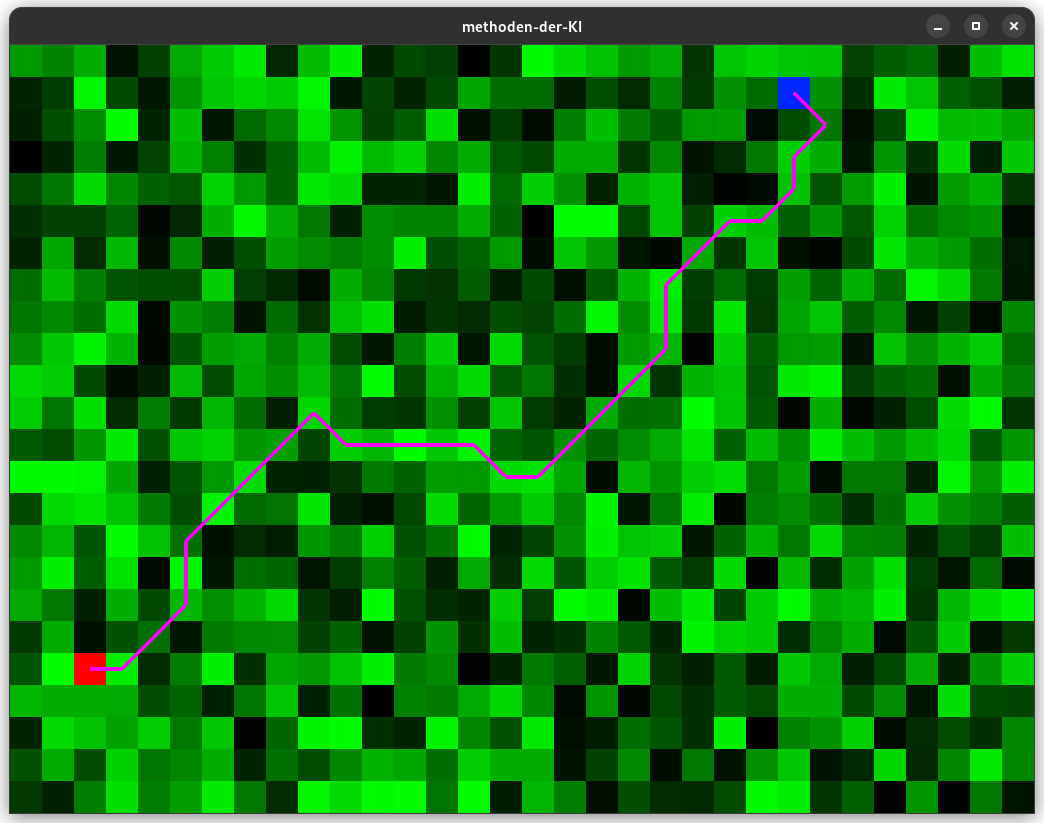
\includegraphics[width=\textwidth]{figures/kap3/a-star-impl.png}
    \caption{Der A*-Pfadfindungs-Screen}
    \label{fig:impl-a-star-pathfinding}
\end{figure}

Bei der Umsetzung wird ein zuf�lliges Terrain in Form von gr�nen Quadraten erzeugt. Je dunkler das Quadrat ist, desto h�her sind die Kosten f�r die Durchquerung des Quadrats. Die Wegfindung beginnt beim roten Quadrat und endet beim blauen Quadrat.

Auf dem A*-Pfadfindungs-Screen des Programms sind die Tastensteuerungen wie folgt:
\begin{itemize}
    \item \textbf{Leertaste:} Erzeugt neues zuf�lliges Terrain und zuf�llige Start- und Endpositionen (Erzeugt eine neue Pfadfindungsaufgabe). 
    \item \textbf{Eingabetaste:} Startet den A*-Pfadfindungsprozess. Der gefundene Pfad wird auf dem SCreen in Form einer hellvioletten Linie angezeigt.
    \item \textbf{Escape-Taste:} Geht zur�ck zum Start-Screen.
\end{itemize}

Es gibt einen Bug im Programm, wodurch manchmal ein Pfad nicht gefunden werden konnte, wenn sich das Ziel am Rand befindet. In diesem Fall wird oben links im Fenster die Meldung ``No traversable route found'' angezeigt.

Der relevante Code f�r das Programm befindet sich in den folgenden Packages (Implementierungscode befindet sich im ``core'' Verzeichnis):
\begin{itemize}
    \item \textbf{de.augsburg.hs.methoden.ki.screens.astar:} Der Code f�r den A-Star-Pathfinding-Screen. Hier kommt der gesamte Code zusammen.
    \item \textbf{de.augsburg.hs.methoden.ki.algorithms.astar:} Allgemeine Implementierung des A*-Wegfindungsalgorithmus.
    \item \textbf{de.augsburg.hs.methoden.ki.algorithms.astar.implementation:} Implementierung des allgemeinen Algorithmus f�r dieses Programm.
    \item \textbf{de.augsburg.hs.methoden.ki.actors.astar:} Enth�lt nur die beiden Actors zum Anzeigen der Start- und Zielquadrate.
\end{itemize}
% \include{einleitung}
% \include{unternehmen}

% \include{projekt_a}
% \include{stellungnahme}

%\include{beispiele}   % Beispiele
%\include{beispiele2}     % Beispiele2

%\chapter*{Hinweis Literatur}
Beachten Sie, dass auch in einem Praxisbericht alle verwendeten Quellen eindeutig gekennzeichnet sein m�ssen. Insbesondere m�ssen Sie auch Bildquellen angeben (sofern Sie die Bilder nicht selbst aufgenommen/erstellt haben). Ebenso muss die Verwendung von Inhalten aus Firmenpr�sentationen angegeben werden. Der Bezug der Textstelle zur Quelle muss eindeutig sein.

Vermeiden Sie die Angabe von Webseiten als Quellen. Wenn Sie diese dennoch verwenden wollen, achten Sie auf eine Angabe der URL mit Abrufdatum und erg�nzen Sie die Quelle falls m�glich mit Autor und Titel.


%% ++++++++++++++++++++++++++++++++++++++++++
%% Anhang
%% ++++++++++++++++++++++++++++++++++++++++++

%\appendix
%\include{anhang_a}
%\include{anhang_b}

%\ifnotonesideelse{\cleardoublepage}{}

%% ++++++++++++++++++++++++++++++++++++++++++
%% Literatur
%% ++++++++++++++++++++++++++++++++++++++++++
\addcontentsline{toc}{chapter}{\bibname}
%  mit dem Befehl \nocite werden auch nicht zitierte Referenzen abgedruckt 
% (normalerweise nicht erwünscht)
% \nocite{*}
\bibliographystyle{rialpha}
%Einbinden Bibtexdatei - Direkt aus JabRef generiert
\bibliography{literatur}
%% ++++++++++++++++++++++++++++++++++++++++++
%% Index (optional)
%% ++++++++++++++++++++++++++++++++++++++++++
%\ifnotdraft{
%\addcontentsline{toc}{chapter}{Index}
%\printindex            % Index, Stichwortverzeichnis
%}
\end{document}
